%\VignetteIndexEntry{The chromstaR users guide}
%\VignetteDepends{chromstaR}
%\VignetteKeywords{ChIP-seq}
%\VignettePackage{chromstaR}
\documentclass[11pt]{article}\usepackage[]{graphicx}\usepackage[]{color}
%% maxwidth is the original width if it is less than linewidth
%% otherwise use linewidth (to make sure the graphics do not exceed the margin)
\makeatletter
\def\maxwidth{ %
  \ifdim\Gin@nat@width>\linewidth
    \linewidth
  \else
    \Gin@nat@width
  \fi
}
\makeatother

\definecolor{fgcolor}{rgb}{0.345, 0.345, 0.345}
\newcommand{\hlnum}[1]{\textcolor[rgb]{0.686,0.059,0.569}{#1}}%
\newcommand{\hlstr}[1]{\textcolor[rgb]{0.192,0.494,0.8}{#1}}%
\newcommand{\hlcom}[1]{\textcolor[rgb]{0.678,0.584,0.686}{\textit{#1}}}%
\newcommand{\hlopt}[1]{\textcolor[rgb]{0,0,0}{#1}}%
\newcommand{\hlstd}[1]{\textcolor[rgb]{0.345,0.345,0.345}{#1}}%
\newcommand{\hlkwa}[1]{\textcolor[rgb]{0.161,0.373,0.58}{\textbf{#1}}}%
\newcommand{\hlkwb}[1]{\textcolor[rgb]{0.69,0.353,0.396}{#1}}%
\newcommand{\hlkwc}[1]{\textcolor[rgb]{0.333,0.667,0.333}{#1}}%
\newcommand{\hlkwd}[1]{\textcolor[rgb]{0.737,0.353,0.396}{\textbf{#1}}}%

\usepackage{framed}
\makeatletter
\newenvironment{kframe}{%
 \def\at@end@of@kframe{}%
 \ifinner\ifhmode%
  \def\at@end@of@kframe{\end{minipage}}%
  \begin{minipage}{\columnwidth}%
 \fi\fi%
 \def\FrameCommand##1{\hskip\@totalleftmargin \hskip-\fboxsep
 \colorbox{shadecolor}{##1}\hskip-\fboxsep
     % There is no \\@totalrightmargin, so:
     \hskip-\linewidth \hskip-\@totalleftmargin \hskip\columnwidth}%
 \MakeFramed {\advance\hsize-\width
   \@totalleftmargin\z@ \linewidth\hsize
   \@setminipage}}%
 {\par\unskip\endMakeFramed%
 \at@end@of@kframe}
\makeatother

\definecolor{shadecolor}{rgb}{.97, .97, .97}
\definecolor{messagecolor}{rgb}{0, 0, 0}
\definecolor{warningcolor}{rgb}{1, 0, 1}
\definecolor{errorcolor}{rgb}{1, 0, 0}
\newenvironment{knitrout}{}{} % an empty environment to be redefined in TeX

\usepackage{alltt}
\usepackage{hyperref}
\usepackage{url}
\usepackage[authoryear,round]{natbib}
\bibliographystyle{plainnat}

\newcommand{\scscst}{\scriptscriptstyle}
\newcommand{\scst}{\scriptstyle}

\newcommand{\Rfunction}[1]{{\texttt{#1}}}
\newcommand{\Robject}[1]{{\texttt{#1}}}
\newcommand{\Rpackage}[1]{{\textit{#1}}}

\author{Aaron Taudt\footnote{a.s.taudt@umcg.nl}}
\IfFileExists{upquote.sty}{\usepackage{upquote}}{}
\begin{document}
\title{The chromstaR user's guide}

\maketitle

\tableofcontents
%%%%%%%%%%%%%%%%%%%%%%%%%%%%%%%%%%%%%%%%%%%%%%%%%%%%%%%%%%%%%%%%%%%%%%%%%%%%%%%
\section{Introduction}

ChIP-seq has become the standard technique for assessing the genome-wide chromatin state of DNA. \Rpackage{chromstaR} provides functions for the joint analysis of multiple ChIP-seq samples. It allows peak calling for transcription factor binding and histone modifications with a narrow (e.g. H3K4me3, H3K27ac,~...) or broad (e.g. H3K36me3, H3K27me3,~...) profile. All analysis can be performed on each sample individually (=univariate), or in a joint analysis considering all samples simultaneously (=multivariate).



\section{Outline of workflow}

Every analysis with the \Rpackage{chromstaR} package starts from aligned reads in either BAM or BED format. In the first step, the genome is partitioned into non-overlapping, equally sized bins and the reads that fall into each bin are counted. These read counts serve as the basis for both the univariate and the multivariate peak- and broad-region calling. Univariate peak calling is done by fitting a three-state Hidden Markov Model to the binned read counts. Multivariate peak calling for $\mathcal{S}$ samples is done by fitting a $2^\mathcal{S}$-state Hidden Markov Model to all binned read counts.

\section{Univariate analysis}

\subsection{\label{sec:narrow}Task 1: Peak calling for a narrow histone modification}

Examples of histone modifications with a narrow profile are H3K4me3, H3K9ac and H3K27ac. For such peak-like modifications, the bin size should be set to a value between 200bp and 1000bp.

If you want to do this example starting from a BAM file, you should have the \Rpackage{chromstaRExampleData} package installed. Otherwise you can skip the first step (Binning) and start from already binned data. If your input is in BED format, use function \Rfunction{bed2binned} instead. Please refer to the FAQ section \ref{sec:faq} for more details and troubleshooting on the binning step.

\begin{scriptsize}
\begin{knitrout}
\definecolor{shadecolor}{rgb}{0.969, 0.969, 0.969}\color{fgcolor}\begin{kframe}
\begin{alltt}
\hlkwd{library}\hlstd{(chromstaR)}
\end{alltt}
\end{kframe}
\end{knitrout}

\begin{knitrout}
\definecolor{shadecolor}{rgb}{0.969, 0.969, 0.969}\color{fgcolor}\begin{kframe}
\begin{alltt}
\hlcom{## === Step 1: Binning ===}
\hlcom{# We use bin size 1000bp and chromosome 12 to keep the example quick}
\hlkwd{library}\hlstd{(chromstaRExampleData)}
\hlstd{bamfile} \hlkwb{<-} \hlkwd{getExampleFilesBAM}\hlstd{(}\hlstr{'H3K4me3'}\hlstd{)[}\hlnum{1}\hlstd{]}
\hlstd{binned.data} \hlkwb{<-} \hlkwd{bam2binned}\hlstd{(bamfile,} \hlkwc{bamindex}\hlstd{=bamfile,} \hlkwc{binsize}\hlstd{=}\hlnum{1000}\hlstd{,}
                          \hlkwc{chromosomes}\hlstd{=}\hlstr{'chr12'}\hlstd{)}
\end{alltt}
\end{kframe}
\end{knitrout}

\begin{knitrout}
\definecolor{shadecolor}{rgb}{0.969, 0.969, 0.969}\color{fgcolor}\begin{kframe}
\begin{alltt}
\hlcom{## === Step 2: Peak calling ===}
\hlcom{# We load the binned.data from step 1 (this is only necessary if step 1 was skipped)}
\hlkwd{data}\hlstd{(}\hlstr{"liver-H3K4me3-BN-male-bio2-tech1_chr12.bam_binsize_1000"}\hlstd{)}
\hlcom{# We restrict the peak calling to 60 seconds to keep this example quick.}
\hlstd{model} \hlkwb{<-} \hlkwd{callPeaksUnivariate}\hlstd{(binned.data,} \hlkwc{ID}\hlstd{=}\hlstr{'H3K4me3'}\hlstd{,} \hlkwc{max.time}\hlstd{=}\hlnum{60}\hlstd{)}
\end{alltt}


{\ttfamily\noindent\itshape\color{messagecolor}{\#\# Replaced read counts > 163 (99.9\% quantile) by 163 in 46 bins. Set option 'read.cutoff.quantile=1' to disable this filtering. This filtering was done to increase the speed of the HMM and should not affect the results.\\\#\# ------------------------------------ Try 1 of 1 -------------------------------------}}\begin{verbatim}
## HMM: number of states = 3
## HMM: number of bins = 46782
## HMM: maximum number of iterations = none
## HMM: maximum running time = 60 sec
## HMM: epsilon = 0.01
## HMM: data mean = 2.47595, data variance = 180.327
##  Iteration              log(P)             dlog(P)     Diff in state 2    Time in sec
##          0                -inf                   -                   -              0
##          1       -60305.655970                 inf               27150              0
##          2       -57564.343441         2741.312529                7264              0
##          3       -55096.051255         2468.292186               16265              1
##          4       -52988.546150         2107.505105               20857              1
##          5       -51902.355623         1086.190527               22596              1
##          6       -51338.505648          563.849975               23479              1
##          7       -50973.526659          364.978988               23880              1
##          8       -50728.674826          244.851834               24059              1
##          9       -50564.458905          164.215921               24127              1
##         10       -50452.182115          112.276790               24142              1
##         11       -50372.874829           79.307286               24146              1
##         12       -50314.763998           58.110831               24143              1
##         13       -50270.651510           44.112488               24131              1
##         14       -50236.102522           34.548987               24123              1
##         15       -50208.329223           27.773299               24113              1
##         16       -50185.529102           22.800121               24094              1
##         17       -50166.497632           19.031470               24080              1
##         18       -50150.401361           16.096271               24058              1
##         19       -50136.643601           13.757760               24047              1
##  Iteration              log(P)             dlog(P)     Diff in state 2    Time in sec
##         20       -50124.783554           11.860047               24030              1
##         21       -50114.486497           10.297056               24020              1
##         22       -50105.492269            8.994229               24013              1
##         23       -50097.594721            7.897548               24000              1
##         24       -50090.627913            6.966808               23988              1
##         25       -50084.456538            6.171375               23984              1
##         26       -50078.969086            5.487452               23974              1
##         27       -50074.072840            4.896246               23964              1
##         28       -50069.690119            4.382721               23951              1
##         29       -50065.755412            3.934707               23942              1
##         30       -50062.213144            3.542267               23935              1
##         31       -50059.015925            3.197219               23927              1
##         32       -50056.123147            2.892779               23919              1
##         33       -50053.499857            2.623289               23917              1
##         34       -50051.115853            2.384004               23903              1
##         35       -50048.944929            2.170924               23889              1
##         36       -50046.964269            1.980660               23879              1
##         37       -50045.153939            1.810330               23871              1
##         38       -50043.496467            1.657472               23869              1
##         39       -50041.976491            1.519976               23867              1
##  Iteration              log(P)             dlog(P)     Diff in state 2    Time in sec
##         40       -50040.580464            1.396027               23859              1
##         41       -50039.296410            1.284054               23853              1
##         42       -50038.113710            1.182700               23851              1
##         43       -50037.022926            1.090784               23846              1
##         44       -50036.015649            1.007277               23842              1
##         45       -50035.084370            0.931278               23836              1
##         46       -50034.222371            0.861999               23830              1
##         47       -50033.423626            0.798746               23824              1
##         48       -50032.682718            0.740908               23818              1
##         49       -50031.994772            0.687946               23817              1
##         50       -50031.355391            0.639381               23813              1
##         51       -50030.760601            0.594790               23811              1
##         52       -50030.206804            0.553796               23811              1
##         53       -50029.690741            0.516064               23809              1
##         54       -50029.209449            0.481292               23806              1
##         55       -50028.760235            0.449214               23801              1
##         56       -50028.340647            0.419588               23796              1
##         57       -50027.948448            0.392199               23795              1
##         58       -50027.581594            0.366854               23793              1
##         59       -50027.238217            0.343377               23788              1
##  Iteration              log(P)             dlog(P)     Diff in state 2    Time in sec
##         60       -50026.916606            0.321611               23783              1
##         61       -50026.615192            0.301414               23780              1
##         62       -50026.332535            0.282658               23778              1
##         63       -50026.067310            0.265225               23776              1
##         64       -50025.818300            0.249010               23776              1
##         65       -50025.584381            0.233918               23774              1
##         66       -50025.364519            0.219862               23774              1
##         67       -50025.157756            0.206763               23773              1
##         68       -50024.963208            0.194548               23772              1
##         69       -50024.780055            0.183153               23768              1
##         70       -50024.607537            0.172518               23766              1
##         71       -50024.444948            0.162589               23764              1
##         72       -50024.291631            0.153318               23764              1
##         73       -50024.146972            0.144659               23764              1
##         74       -50024.010399            0.136573               23763              1
##         75       -50023.881376            0.129023               23760              1
##         76       -50023.759399            0.121977               23759              1
##         77       -50023.643994            0.115404               23759              1
##         78       -50023.534715            0.109279               23756              1
##         79       -50023.431137            0.103578               23751              1
##  Iteration              log(P)             dlog(P)     Diff in state 2    Time in sec
##         80       -50023.332859            0.098278               23749              1
##         81       -50023.239497            0.093361               23745              1
##         82       -50023.150690            0.088808               23745              1
##         83       -50023.066089            0.084600               23744              1
##         84       -50022.985369            0.080720               23744              1
##         85       -50022.908221            0.077149               23741              1
##         86       -50022.834357            0.073864               23741              1
##         87       -50022.763517            0.070841               23740              1
##         88       -50022.695466            0.068051               23740              1
##         89       -50022.630005            0.065461               23740              1
##         90       -50022.566973            0.063033               23740              1
##         91       -50022.506246            0.060727               23739              1
##         92       -50022.447744            0.058502               23738              1
##         93       -50022.391427            0.056317               23738              1
##         94       -50022.337287            0.054140               23738              1
##         95       -50022.285342            0.051945               23736              1
##         96       -50022.235625            0.049717               23736              1
##         97       -50022.188172            0.047453               23735              1
##         98       -50022.143011            0.045161               23735              1
##         99       -50022.100153            0.042858               23735              1
##  Iteration              log(P)             dlog(P)     Diff in state 2    Time in sec
##        100       -50022.059587            0.040567               23734              1
##        101       -50022.021274            0.038312               23733              1
##        102       -50021.985156            0.036118               23732              1
##        103       -50021.951151            0.034005               23731              1
##        104       -50021.919162            0.031989               23731              1
##        105       -50021.889081            0.030081               23731              1
##        106       -50021.860794            0.028287               23729              1
##        107       -50021.834185            0.026608               23729              1
##        108       -50021.809142            0.025044               23729              1
##        109       -50021.785554            0.023588               23728              1
##        110       -50021.763317            0.022236               23728              2
##        111       -50021.742336            0.020981               23725              2
##        112       -50021.722520            0.019816               23725              2
##        113       -50021.703787            0.018733               23724              2
##        114       -50021.686063            0.017724               23722              2
##        115       -50021.669278            0.016785               23722              2
##        116       -50021.653371            0.015907               23722              2
##        117       -50021.638284            0.015087               23720              2
##        118       -50021.623965            0.014318               23719              2
##        119       -50021.610368            0.013597               23719              2
##  Iteration              log(P)             dlog(P)     Diff in state 2    Time in sec
##        120       -50021.597449            0.012919               23719              2
##        121       -50021.585168            0.012281               23719              2
##        122       -50021.573488            0.011680               23718              2
##        123       -50021.562375            0.011112               23718              2
##        124       -50021.551800            0.010576               23718              2
##        125       -50021.541731            0.010068               23717              2
##        126       -50021.532143            0.009588               23715              2
## HMM: Convergence reached!
## HMM: Recoding posteriors ...
\end{verbatim}


{\ttfamily\noindent\itshape\color{messagecolor}{\#\# Calculating states from posteriors ... 0.24s\\\#\# Making segmentation ... 0.44s}}\end{kframe}
\end{knitrout}

\begin{knitrout}
\definecolor{shadecolor}{rgb}{0.969, 0.969, 0.969}\color{fgcolor}\begin{kframe}
\begin{alltt}
\hlcom{## === Step 3: Checking the fit ===}
\hlcom{# For a narrow modification, the fit should look something like this,}
\hlcom{# with the 'modified'-component near the bottom of the figure}
\hlkwd{plot}\hlstd{(model)}
\end{alltt}
\end{kframe}
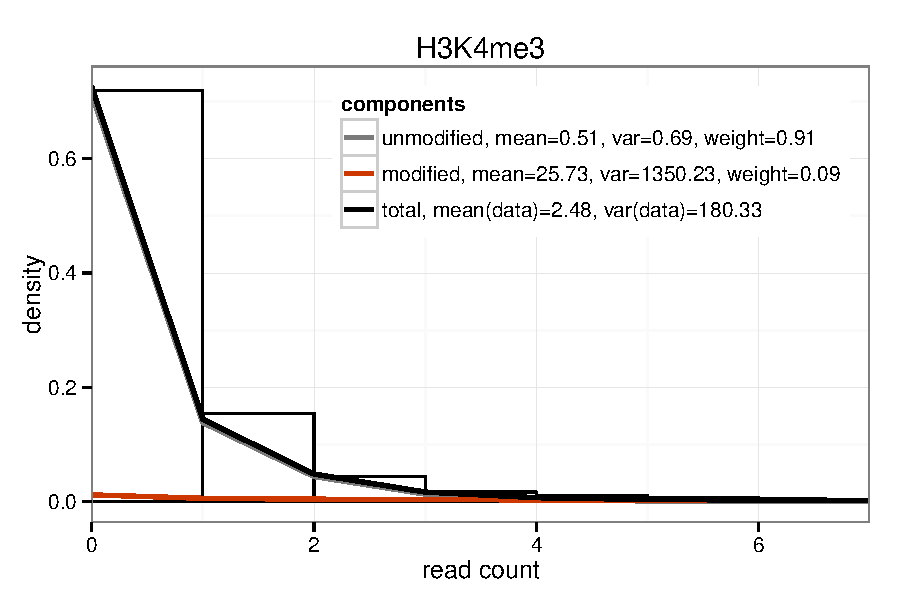
\includegraphics[width=\maxwidth]{figure/univariate_narrow_plotting-1} 

\end{knitrout}

\begin{knitrout}
\definecolor{shadecolor}{rgb}{0.969, 0.969, 0.969}\color{fgcolor}\begin{kframe}
\begin{alltt}
\hlcom{## === Step 4: Export to genome browser ===}
\hlcom{# We can export peak calls and binned read counts with}
\hlkwd{exportUnivariates}\hlstd{(}\hlkwd{list}\hlstd{(model),} \hlkwc{filename}\hlstd{=}\hlstr{'your-file'}\hlstd{,} \hlkwc{what}\hlstd{=}\hlkwd{c}\hlstd{(}\hlstr{'peaks'}\hlstd{,}\hlstr{'reads'}\hlstd{))}
\end{alltt}
\end{kframe}
\end{knitrout}
\end{scriptsize}

\subsection{\label{sec:broad}Task 2: Peak calling for a broad histone modification}

Examples of histone modifications with a broad profile are H3K9me3, H3K27me3, H3K36me3, H4K20me1. These modifications usually cover broad domains of the genome, and the enrichment is best captured with a bin size between 500bp and 2000bp.

If you want to do this example starting from a BAM file, you should have the \Rpackage{chromstaRExampleData} package installed. Otherwise you can skip the first step (Binning) and start from already binned data. If your input is in BED format, use function \Rfunction{bed2binned} instead. Please refer to the FAQ section \ref{sec:faq} for more details and troubleshooting on the binning step.

\begin{scriptsize}
\begin{knitrout}
\definecolor{shadecolor}{rgb}{0.969, 0.969, 0.969}\color{fgcolor}\begin{kframe}
\begin{alltt}
\hlkwd{library}\hlstd{(chromstaR)}
\end{alltt}
\end{kframe}
\end{knitrout}

\begin{knitrout}
\definecolor{shadecolor}{rgb}{0.969, 0.969, 0.969}\color{fgcolor}\begin{kframe}
\begin{alltt}
\hlcom{## === Step 1: Binning ===}
\hlcom{# We use bin size 1000bp and chromosome 12 to keep the example quick}
\hlkwd{library}\hlstd{(chromstaRExampleData)}
\hlstd{bamfile} \hlkwb{<-} \hlkwd{getExampleFilesBAM}\hlstd{(}\hlstr{'H3K27me3'}\hlstd{)[}\hlnum{4}\hlstd{]}
\hlstd{binned.data} \hlkwb{<-} \hlkwd{bam2binned}\hlstd{(bamfile,} \hlkwc{bamindex}\hlstd{=bamfile,} \hlkwc{binsize}\hlstd{=}\hlnum{1000}\hlstd{,}
                          \hlkwc{chromosomes}\hlstd{=}\hlstr{'chr12'}\hlstd{)}
\end{alltt}
\end{kframe}
\end{knitrout}

\begin{knitrout}
\definecolor{shadecolor}{rgb}{0.969, 0.969, 0.969}\color{fgcolor}\begin{kframe}
\begin{alltt}
\hlcom{## === Step 2: Peak calling ===}
\hlcom{# We load the binned.data from step 1 (this is only necessary if step 1 was skipped)}
\hlkwd{data}\hlstd{(}\hlstr{"liver-H3K27me3-BN-male-bio3-tech1_chr12.bam_binsize_1000"}\hlstd{)}
\hlcom{# We restrict the peak calling to 60 seconds to keep this example quick.}
\hlstd{model} \hlkwb{<-} \hlkwd{callPeaksUnivariate}\hlstd{(binned.data,} \hlkwc{ID}\hlstd{=}\hlstr{'H3K27me3'}\hlstd{,} \hlkwc{max.time}\hlstd{=}\hlnum{60}\hlstd{)}
\end{alltt}


{\ttfamily\noindent\itshape\color{messagecolor}{\#\# Replaced read counts > 70 (99.9\% quantile) by 70 in 44 bins. Set option 'read.cutoff.quantile=1' to disable this filtering. This filtering was done to increase the speed of the HMM and should not affect the results.\\\#\# ------------------------------------ Try 1 of 1 -------------------------------------}}\begin{verbatim}
## HMM: number of states = 3
## HMM: number of bins = 46782
## HMM: maximum number of iterations = none
## HMM: maximum running time = 60 sec
## HMM: epsilon = 0.01
## HMM: data mean = 9.9711, data variance = 115.938
##  Iteration              log(P)             dlog(P)     Diff in state 2    Time in sec
##          0                -inf                   -                   -              0
##          1      -145371.198541                 inf               26373              0
##          2      -138286.718658         7084.479883                4015              0
##          3      -135011.421891         3275.296767                3861              0
##          4      -133645.293004         1366.128887                3349              0
##          5      -132693.106686          952.186318                2935              0
##          6      -132053.945399          639.161287                2638              0
##          7      -131618.103384          435.842015                2443              0
##          8      -131313.355266          304.748118                2313              0
##          9      -131094.488639          218.866627                2234              0
##         10      -130933.648422          160.840217                2154              0
##         11      -130813.261091          120.387331                2110              0
##         12      -130721.783983           91.477108                2067              0
##         13      -130651.375524           70.408459                2045              0
##         14      -130596.576783           54.798740                2036              0
##         15      -130553.513780           43.063004                2024              0
##         16      -130519.389828           34.123952                2021              0
##         17      -130492.153400           27.236428                2027              0
##         18      -130470.277142           21.876257                2013              0
##         19      -130452.608676           17.668467                2008              0
##  Iteration              log(P)             dlog(P)     Diff in state 2    Time in sec
##         20      -130438.268226           14.340450                2010              0
##         21      -130426.577202           11.691025                2012              0
##         22      -130417.007491            9.569711                1994              0
##         23      -130409.144899            7.862592                1991              0
##         24      -130402.662365            6.482534                1987              0
##         25      -130397.300088            5.362276                1989              0
##         26      -130392.850605            4.449483                1992              0
##         27      -130389.147463            3.703143                1983              0
##         28      -130386.056541            3.090922                1982              0
##         29      -130383.469355            2.587186                1978              0
##         30      -130381.297844            2.171511                1969              0
##         31      -130379.470292            1.827552                1974              0
##         32      -130377.928115            1.542176                1976              0
##         33      -130376.623323            1.304793                1969              0
##         34      -130375.516493            1.106830                1968              0
##         35      -130374.575161            0.941331                1961              0
##         36      -130373.772528            0.802634                1958              0
##         37      -130373.086413            0.686115                1955              0
##         38      -130372.498423            0.587990                1956              0
##         39      -130371.993265            0.505158                1952              0
##  Iteration              log(P)             dlog(P)     Diff in state 2    Time in sec
##         40      -130371.558199            0.435066                1948              0
##         41      -130371.182588            0.375611                1944              0
##         42      -130370.857530            0.325058                1944              0
##         43      -130370.575559            0.281971                1942              1
##         44      -130370.330401            0.245158                1941              1
##         45      -130370.116770            0.213630                1937              1
##         46      -130369.930206            0.186564                1933              1
##         47      -130369.766934            0.163272                1930              1
##         48      -130369.623753            0.143181                1928              1
##         49      -130369.497942            0.125811                1928              1
##         50      -130369.387185            0.110758                1927              1
##         51      -130369.289502            0.097683                1925              1
##         52      -130369.203201            0.086301                1924              1
##         53      -130369.126830            0.076371                1923              1
##         54      -130369.059139            0.067690                1923              1
##         55      -130368.999054            0.060085                1921              1
##         56      -130368.945645            0.053409                1918              1
##         57      -130368.898107            0.047538                1919              1
##         58      -130368.855742            0.042364                1917              1
##         59      -130368.817945            0.037798                1917              1
##  Iteration              log(P)             dlog(P)     Diff in state 2    Time in sec
##         60      -130368.784185            0.033760                1917              1
##         61      -130368.754001            0.030184                1915              1
##         62      -130368.726988            0.027012                1913              1
##         63      -130368.702793            0.024195                1912              1
##         64      -130368.681104            0.021689                1913              1
##         65      -130368.661646            0.019458                1910              1
##         66      -130368.644178            0.017468                1910              1
##         67      -130368.628487            0.015691                1910              1
##         68      -130368.614382            0.014104                1909              1
##         69      -130368.601698            0.012684                1909              1
##         70      -130368.590285            0.011413                1908              1
##         71      -130368.580012            0.010274                1909              1
##         72      -130368.570759            0.009252                1907              1
## HMM: Convergence reached!
## HMM: Recoding posteriors ...
\end{verbatim}


{\ttfamily\noindent\itshape\color{messagecolor}{\#\# Calculating states from posteriors ... 0.03s\\\#\# Making segmentation ... 0.41s}}\end{kframe}
\end{knitrout}

\begin{knitrout}
\definecolor{shadecolor}{rgb}{0.969, 0.969, 0.969}\color{fgcolor}\begin{kframe}
\begin{alltt}
\hlcom{## === Step 3: Checking the fit ===}
\hlcom{# For a broad modification, the fit should look something like this,}
\hlcom{# with a 'modified'-component that fits the thick tail of the distribution.}
\hlkwd{plot}\hlstd{(model)}
\end{alltt}
\end{kframe}
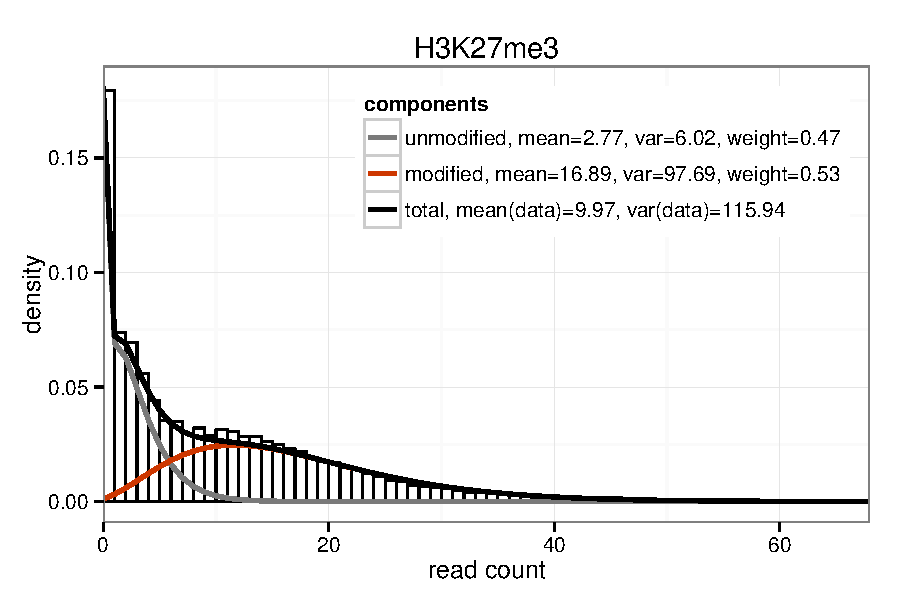
\includegraphics[width=\maxwidth]{figure/univariate_broad_plotting-1} 

\end{knitrout}

\begin{knitrout}
\definecolor{shadecolor}{rgb}{0.969, 0.969, 0.969}\color{fgcolor}
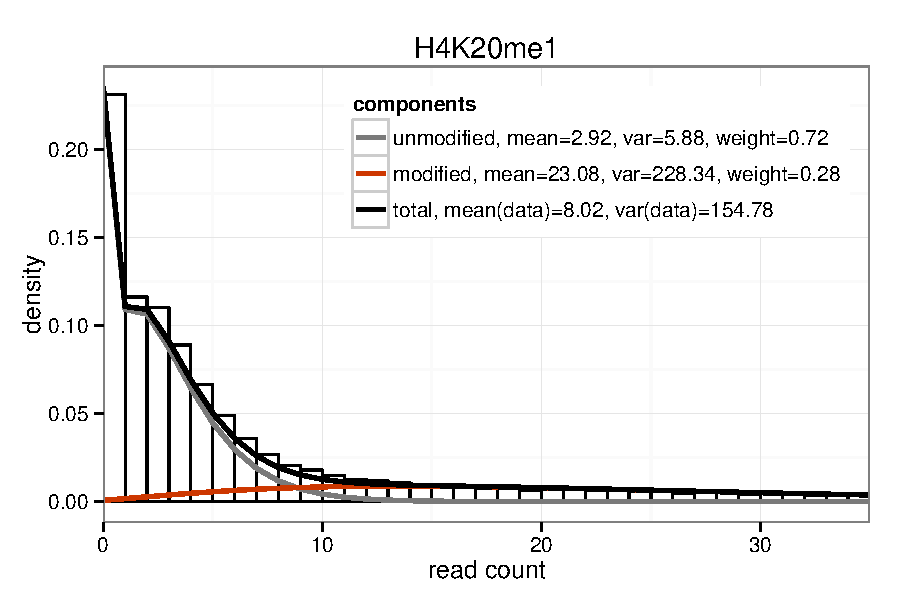
\includegraphics[width=\maxwidth]{figure/univariate_broad_H4K20me1-1} 

\end{knitrout}

\begin{knitrout}
\definecolor{shadecolor}{rgb}{0.969, 0.969, 0.969}\color{fgcolor}\begin{kframe}
\begin{alltt}
\hlcom{## === Step 4: Export to genome browser ===}
\hlcom{# We can export peak calls and binned read counts with}
\hlkwd{exportUnivariates}\hlstd{(}\hlkwd{list}\hlstd{(model),} \hlkwc{filename}\hlstd{=}\hlstr{'your-file'}\hlstd{,} \hlkwc{what}\hlstd{=}\hlkwd{c}\hlstd{(}\hlstr{'peaks'}\hlstd{,}\hlstr{'reads'}\hlstd{))}
\end{alltt}
\end{kframe}
\end{knitrout}
\end{scriptsize}

\subsection{Task 3: Peak calling for ATAC-seq, DNase-seq, FAIRE-seq, ...}

Peak calling for ATAC-seq and DNase-seq is similar to the peak calling of a narrow histone modification (see section~\ref{sec:narrow}). FAIRE-seq experiments seem to exhibit a broad profile with our model, so the procedure is similar to the domain calling of a broad histone modification (see section~\ref{sec:broad}).

\section{Multivariate analysis}
\subsection{Task 1: Integrating multiple replicates}

\Rpackage{chromstaR} can be used to call peaks with multiple replicates, without the need of prior merging. The underlying statistical model integrates information from all replicates to identify common peaks. It is, however, important to note that replicates with poor quality can affect the joint peak calling negatively. It is therefore recommended to first check the replicate quality and discard poor-quality replicates. The necessary steps for peak calling for an example ChIP-seq experiment with 4 replicates are detailed below.

\begin{scriptsize}
\begin{knitrout}
\definecolor{shadecolor}{rgb}{0.969, 0.969, 0.969}\color{fgcolor}\begin{kframe}
\begin{alltt}
\hlkwd{library}\hlstd{(chromstaR)}
\end{alltt}
\end{kframe}
\end{knitrout}

\begin{knitrout}
\definecolor{shadecolor}{rgb}{0.969, 0.969, 0.969}\color{fgcolor}\begin{kframe}
\begin{alltt}
\hlcom{## === Step 1: Binning ===}
\hlcom{# !!! Skip this step if you do not have package 'chromstaRExampleData' installed !!!}
\hlkwd{library}\hlstd{(chromstaRExampleData)}
\hlcom{# Let's get some example data with 3 replicates}
\hlstd{bamfiles.good} \hlkwb{<-} \hlkwd{getExampleFilesBAM}\hlstd{(}\hlstr{'H3K27me3'}\hlstd{)[}\hlnum{3}\hlopt{:}\hlnum{5}\hlstd{]}
\hlcom{# We fake a replicate with poor quality by taking a different mark entirely}
\hlstd{bamfiles.poor} \hlkwb{<-} \hlkwd{getExampleFilesBAM}\hlstd{(}\hlstr{'H4K20me1'}\hlstd{)[}\hlnum{1}\hlstd{]}
\hlstd{bamfiles} \hlkwb{<-} \hlkwd{c}\hlstd{(bamfiles.good, bamfiles.poor)}
\hlcom{# We use bin size 1000bp and chromosome 12 to keep the example quick}
\hlstd{binned.data} \hlkwb{<-} \hlkwd{list}\hlstd{()}
\hlkwa{for} \hlstd{(bamfile} \hlkwa{in} \hlstd{bamfiles) \{}
  \hlstd{binned.data[[}\hlkwd{basename}\hlstd{(bamfile)]]} \hlkwb{<-} \hlkwd{bam2binned}\hlstd{(bamfile,} \hlkwc{bamindex}\hlstd{=bamfile,}
                                                 \hlkwc{binsize}\hlstd{=}\hlnum{1000}\hlstd{,} \hlkwc{chromosomes}\hlstd{=}\hlstr{'chr12'}\hlstd{)}
\hlstd{\}}
\end{alltt}
\end{kframe}
\end{knitrout}

\begin{knitrout}
\definecolor{shadecolor}{rgb}{0.969, 0.969, 0.969}\color{fgcolor}\begin{kframe}
\begin{alltt}
\hlcom{## === Step 2: Univariate peak calling ===}
\hlcom{# We load the binned.data from step 1 (this is only necessary if step 1 was skipped)}
\hlkwd{data}\hlstd{(replicateExample_binnedData)}
\hlcom{# The univariate fit is obtained for each replicate}
\hlstd{models} \hlkwb{<-} \hlkwd{list}\hlstd{()}
\hlkwa{for} \hlstd{(i1} \hlkwa{in} \hlnum{1}\hlopt{:}\hlkwd{length}\hlstd{(binned.data)) \{}
  \hlstd{models[[i1]]} \hlkwb{<-} \hlkwd{callPeaksUnivariate}\hlstd{(binned.data[[i1]],} \hlkwc{ID}\hlstd{=}\hlkwd{paste0}\hlstd{(}\hlstr{'Rep'}\hlstd{,i1),}
                                      \hlkwc{max.time}\hlstd{=}\hlnum{60}\hlstd{)}
\hlstd{\}}
\end{alltt}
\end{kframe}
\end{knitrout}

\begin{knitrout}
\definecolor{shadecolor}{rgb}{0.969, 0.969, 0.969}\color{fgcolor}\begin{kframe}
\begin{alltt}
\hlcom{## === Step 3: Check replicate correlation ===}
\hlcom{# We run a multivariate peak calling on all 4 replicates}
\hlcom{# A warning is issued because replicate 4 is very different from the others}
\hlstd{multi.model} \hlkwb{<-} \hlkwd{callPeaksReplicates}\hlstd{(models,} \hlkwc{max.time}\hlstd{=}\hlnum{60}\hlstd{)}
\end{alltt}


{\ttfamily\noindent\color{warningcolor}{\#\# Warning in callPeaksReplicates(models, max.time = 60): Your replicates cluster in 2 groups. Consider redoing your analysis with only the group with the highest average coverage:\\\#\# Rep1\\\#\# Rep2\\\#\# Rep3\\\#\# Replicates from groups with lower coverage are:\\\#\# Rep4}}\end{kframe}
\end{knitrout}
\begin{knitrout}
\definecolor{shadecolor}{rgb}{0.969, 0.969, 0.969}\color{fgcolor}\begin{kframe}
\begin{alltt}
\hlcom{# Checking the correlation confirms that Rep4 is very different from the others}
\hlstd{multi.model}\hlopt{$}\hlstd{replicateInfo}\hlopt{$}\hlstd{correlation}
\end{alltt}
\begin{verbatim}
##            Rep1       Rep2       Rep3       Rep4
## Rep1  1.0000000  0.9976476  0.9977751 -0.4126249
## Rep2  0.9976476  1.0000000  0.9984169 -0.4115774
## Rep3  0.9977751  0.9984169  1.0000000 -0.4115570
## Rep4 -0.4126249 -0.4115774 -0.4115570  1.0000000
\end{verbatim}
\end{kframe}
\end{knitrout}

\begin{knitrout}
\definecolor{shadecolor}{rgb}{0.969, 0.969, 0.969}\color{fgcolor}\begin{kframe}
\begin{alltt}
\hlcom{## === Step 4: Peak calling with replicates ===}
\hlcom{# We redo the previous step without the "bad" replicate}
\hlcom{# Also, we force all replicates to agree in their peak calls}
\hlstd{multi.model} \hlkwb{<-} \hlkwd{callPeaksReplicates}\hlstd{(models[}\hlnum{1}\hlopt{:}\hlnum{3}\hlstd{],} \hlkwc{force.equal}\hlstd{=}\hlnum{TRUE}\hlstd{,} \hlkwc{max.time}\hlstd{=}\hlnum{60}\hlstd{)}
\end{alltt}
\end{kframe}
\end{knitrout}

\begin{knitrout}
\definecolor{shadecolor}{rgb}{0.969, 0.969, 0.969}\color{fgcolor}\begin{kframe}
\begin{alltt}
\hlcom{## === Step 5: Export to genome browser ===}
\hlcom{# Finally, we can export the results as BED file}
\hlkwd{exportMultivariate}\hlstd{(multi.model,} \hlkwc{filename}\hlstd{=}\hlstr{'your-file'}\hlstd{,} \hlkwc{what}\hlstd{=}\hlkwd{c}\hlstd{(}\hlstr{'peaks'}\hlstd{,}\hlstr{'reads'}\hlstd{))}
\end{alltt}
\end{kframe}
\end{knitrout}
\end{scriptsize}

\subsection{Task 2: Detecting differentially modified regions}

\Rpackage{chromstaR} is extremely powerful in detecting differentially modified regions in two or more samples. The following example illustrates this on ChIP-seq data for H3K36me3 in 7 different human brain tissues. With 7 samples we can have $2^7 = 128$ combinatorial states, which can be readily interpreted as '0: all samples unmodified', '1-126: DMR' and '127: all samples modified'. Having several replicates for each sample makes it more complicated, but you get the idea ...

\begin{scriptsize}
\begin{knitrout}
\definecolor{shadecolor}{rgb}{0.969, 0.969, 0.969}\color{fgcolor}\begin{kframe}
\begin{alltt}
\hlkwd{library}\hlstd{(chromstaR)}
\end{alltt}
\end{kframe}
\end{knitrout}

\begin{knitrout}
\definecolor{shadecolor}{rgb}{0.969, 0.969, 0.969}\color{fgcolor}\begin{kframe}
\begin{alltt}
\hlcom{## === Step 1: Binning ===}
\hlcom{# !!! Skip this step if you do not have package 'chromstaRExampleData' installed !!!}
\hlkwd{library}\hlstd{(chromstaRExampleData)}
\hlcom{# Let's get some example data with 3 replicates}
\hlstd{bedfiles} \hlkwb{<-} \hlkwd{getExampleFilesBED}\hlstd{()}
\hlcom{# We use bin size 1000bp and chromosome 22 to keep the example quick}
\hlstd{binned.data} \hlkwb{<-} \hlkwd{list}\hlstd{()}
\hlkwa{for} \hlstd{(bedfile} \hlkwa{in} \hlstd{bedfiles) \{}
  \hlstd{binned.data[[}\hlkwd{basename}\hlstd{(bedfile)]]} \hlkwb{<-} \hlkwd{bed2binned}\hlstd{(bedfile,} \hlkwc{assembly}\hlstd{=}\hlstr{'hg19'}\hlstd{,}
                                                 \hlkwc{binsize}\hlstd{=}\hlnum{1000}\hlstd{,} \hlkwc{chromosomes}\hlstd{=}\hlstr{'chr22'}\hlstd{)}
\hlstd{\}}
\end{alltt}
\end{kframe}
\end{knitrout}

\begin{knitrout}
\definecolor{shadecolor}{rgb}{0.969, 0.969, 0.969}\color{fgcolor}\begin{kframe}
\begin{alltt}
\hlcom{## === Step 2: Univariate peak calling ===}
\hlcom{# We load the binned.data from step 1 (this is only necessary if step 1 was skipped)}
\hlkwd{data}\hlstd{(differentialExample_binnedData)}
\hlcom{# The univariate fit is obtained for each sample}
\hlstd{models} \hlkwb{<-} \hlkwd{list}\hlstd{()}
\hlkwa{for} \hlstd{(i1} \hlkwa{in} \hlnum{1}\hlopt{:}\hlkwd{length}\hlstd{(binned.data)) \{}
  \hlkwd{message}\hlstd{(}\hlstr{"Fitting model "}\hlstd{, i1)}
  \hlstd{models[[i1]]} \hlkwb{<-} \hlkwd{callPeaksUnivariate}\hlstd{(binned.data[[i1]],} \hlkwc{ID}\hlstd{=}\hlkwd{names}\hlstd{(binned.data)[i1],}
                                      \hlkwc{max.time}\hlstd{=}\hlnum{60}\hlstd{,} \hlkwc{verbosity}\hlstd{=}\hlnum{0}\hlstd{)}
\hlstd{\}}
\end{alltt}
\end{kframe}
\end{knitrout}

\begin{knitrout}
\definecolor{shadecolor}{rgb}{0.969, 0.969, 0.969}\color{fgcolor}\begin{kframe}
\begin{alltt}
\hlcom{## === Step 3: Constructing the combinatorial states ===}
\hlcom{# This step is only necessary if you have replicates for each sample.}
\hlcom{# To ensure that replicates are treated as such, and not as independent}
\hlcom{# samples, we have to construct the proper combinatorial states:}

\hlcom{# First, we get all the tissues (we could specify them by hand, but we are lazy)}
\hlstd{IDs} \hlkwb{<-} \hlkwd{names}\hlstd{(binned.data)}
\hlstd{tissues} \hlkwb{<-} \hlkwd{unlist}\hlstd{(}\hlkwd{lapply}\hlstd{(}\hlkwd{strsplit}\hlstd{(IDs,} \hlstr{'.Brain_|\textbackslash{}\textbackslash{}.'}\hlstd{),} \hlstr{'[['}\hlstd{,} \hlnum{2}\hlstd{))}
\hlkwd{print}\hlstd{(tissues)}
\end{alltt}
\begin{verbatim}
##  [1] "Angular_Gyrus"          "Angular_Gyrus"         
##  [3] "Anterior_Caudate"       "Anterior_Caudate"      
##  [5] "Cingulate_Gyrus"        "Cingulate_Gyrus"       
##  [7] "Hippocampus_Middle"     "Hippocampus_Middle"    
##  [9] "Inferior_Temporal_Lobe" "Inferior_Temporal_Lobe"
## [11] "Mid_Frontal_Lobe"       "Mid_Frontal_Lobe"      
## [13] "Substantia_Nigra"       "Substantia_Nigra"
\end{verbatim}
\begin{alltt}
\hlcom{# Second, we obtain the combinatorial states}
\hlcom{# Look up ?stateBrewer on how to use this function}
\hlstd{states} \hlkwb{<-} \hlkwd{stateBrewer}\hlstd{(}\hlkwc{statespec} \hlstd{=} \hlkwd{paste0}\hlstd{(}\hlstr{'r.'}\hlstd{, tissues))}
\hlcom{# Third, we construct common states}
\hlstd{common.states} \hlkwb{<-} \hlkwd{c}\hlstd{(}\hlkwd{stateBrewer}\hlstd{(}\hlkwc{statespec} \hlstd{=} \hlkwd{paste0}\hlstd{(}\hlstr{'1.'}\hlstd{, tissues)),}
                   \hlkwd{stateBrewer}\hlstd{(}\hlkwc{statespec} \hlstd{=} \hlkwd{paste0}\hlstd{(}\hlstr{'0.'}\hlstd{, tissues)))}
\end{alltt}
\end{kframe}
\end{knitrout}

\begin{knitrout}
\definecolor{shadecolor}{rgb}{0.969, 0.969, 0.969}\color{fgcolor}\begin{kframe}
\begin{alltt}
\hlcom{## === Step 4: Multivariate peak calling ===}
\hlstd{multi.model} \hlkwb{<-} \hlkwd{callPeaksMultivariate}\hlstd{(models,} \hlkwc{use.states}\hlstd{=states,} \hlkwc{eps}\hlstd{=}\hlnum{1}\hlstd{,} \hlkwc{max.time}\hlstd{=}\hlnum{60}\hlstd{)}
\end{alltt}


{\ttfamily\noindent\itshape\color{messagecolor}{\#\# Extracting reads from modellist... 0.02s\\\#\# Getting combinatorial states... 0.08s\\\#\# Computing pre z-matrix... 0.01s\\\#\# Transfering values into z-matrix... 0.1s\\\#\# Computing inverse of correlation matrix... 4.52s\\\#\# \\\#\# Starting multivariate HMM\\\#\# Using the following combinatorial states, covering 86.8840636207703\% of the bins:\\\#\# 0 16383 3072 16380 192 13116 16371 12 768 3264 12300 13308 3084 15375 3120 3840 4095 15420 16188 3075 16128 16191 3 48 960 3123 3315 3903 4092 12540 15363 15612 16179 15 51 60 63 195 204 207 240 243 252 255 771 780 783 816 819 828 831 963 972 975 1008 1011 1020 1023 3087 3132 3135 3267 3276 3279 3312 3324 3327 3843 3852 3855 3888 3891 3900 4032 4035 4044 4047 4080 4083 12288 12291 12303 12336 12339 12348 12351 12480 12483 12492 12495 12528 12531 12543 13056 13059 13068 13071 13104 13107 13119 13248 13251 13260 13263 13296 13299 13311 15360 15372 15408 15411 15423 15552 15555 15564 15567 15600 15603 15615 16131 16140 16143 16176 16320 16323 16332 16335 16368}}\begin{verbatim}
## HMM: number of states = 128
## HMM: number of bins = 51304
## HMM: maximum number of iterations = none
## HMM: maximum running time = 60 sec
## HMM: epsilon = 1
## HMM: number of modifications = 14
##  Iteration              log(P)             dlog(P)    Time in sec
##          0                -inf                   -              0
## HMM: Precomputing densities ...
##  Iteration              log(P)             dlog(P)    Time in sec
##          0                -inf                   -             13
##          1     -1470427.292494                 inf             20
##          2     -1463343.769468         7083.523026             27
##          3     -1463199.730689          144.038780             33
##          4     -1463181.468977           18.261712             40
##          5     -1463178.007584            3.461393             47
##          6     -1463176.926714            1.080870             54
##          7     -1463176.529079            0.397635             61
## HMM: Convergence reached!
## HMM: Recoding posteriors ...
\end{verbatim}


{\ttfamily\noindent\itshape\color{messagecolor}{\#\# Transforming posteriors to `per sample` representation ... 0.54s\\\#\# Calculating states from posteriors ... 0.01s\\\#\# Making segmentation ... 0.77s}}\end{kframe}
\end{knitrout}

\begin{knitrout}
\definecolor{shadecolor}{rgb}{0.969, 0.969, 0.969}\color{fgcolor}\begin{kframe}
\begin{alltt}
\hlcom{## === Step 5: Export to genome browser ===}
\hlcom{# Export only differential peaks by excluding the 'common.states'}
\hlkwd{exportMultivariate}\hlstd{(multi.model,} \hlkwc{filename}\hlstd{=}\hlstr{'your-file'}\hlstd{,} \hlkwc{what}\hlstd{=}\hlkwd{c}\hlstd{(}\hlstr{'peaks'}\hlstd{,}\hlstr{'reads'}\hlstd{),}
                   \hlkwc{exclude.states}\hlstd{=common.states)}
\end{alltt}
\end{kframe}
\end{knitrout}
\end{scriptsize}

\subsection{Task 3: Finding combinatorial chromatin states}

TODO: Introduction

\begin{scriptsize}
\begin{knitrout}
\definecolor{shadecolor}{rgb}{0.969, 0.969, 0.969}\color{fgcolor}\begin{kframe}
\begin{alltt}
\hlkwd{library}\hlstd{(chromstaR)}
\end{alltt}
\end{kframe}
\end{knitrout}

\begin{knitrout}
\definecolor{shadecolor}{rgb}{0.969, 0.969, 0.969}\color{fgcolor}\begin{kframe}
\begin{alltt}
\hlcom{## === Step 1: Binning ===}
\hlcom{# !!! Skip this step if you do not have package 'chromstaRExampleData' installed !!!}
\hlkwd{library}\hlstd{(chromstaRExampleData)}
\hlcom{# Let's get some example data with 3 replicates}
\hlstd{bamfiles} \hlkwb{<-} \hlkwd{getExampleFilesBAM}\hlstd{()}
\hlcom{# We use bin size 1000bp and chromosome 22 to keep the example quick}
\hlstd{binned.data} \hlkwb{<-} \hlkwd{list}\hlstd{()}
\hlkwa{for} \hlstd{(bamfile} \hlkwa{in} \hlstd{bamfiles) \{}
  \hlstd{binned.data[[}\hlkwd{basename}\hlstd{(bamfile)]]} \hlkwb{<-} \hlkwd{bam2binned}\hlstd{(bamfile,} \hlkwc{bamindex}\hlstd{=bamfile,}
                                                 \hlkwc{binsize}\hlstd{=}\hlnum{1000}\hlstd{,} \hlkwc{chromosomes}\hlstd{=}\hlstr{'chr12'}\hlstd{)}
\hlstd{\}}
\end{alltt}
\end{kframe}
\end{knitrout}

\begin{knitrout}
\definecolor{shadecolor}{rgb}{0.969, 0.969, 0.969}\color{fgcolor}\begin{kframe}
\begin{alltt}
\hlcom{## === Step 2: Univariate peak calling ===}
\hlcom{# We load the binned.data from step 1 (this is only necessary if step 1 was skipped)}
\hlkwd{data}\hlstd{(combinatorialExample_binnedData)}
\hlcom{# The univariate fit is obtained for each sample}
\hlstd{models} \hlkwb{<-} \hlkwd{list}\hlstd{()}
\hlkwa{for} \hlstd{(i1} \hlkwa{in} \hlnum{1}\hlopt{:}\hlkwd{length}\hlstd{(binned.data)) \{}
  \hlkwd{message}\hlstd{(}\hlstr{"Fitting model "}\hlstd{, i1)}
  \hlstd{models[[i1]]} \hlkwb{<-} \hlkwd{callPeaksUnivariate}\hlstd{(binned.data[[i1]],} \hlkwc{ID}\hlstd{=}\hlkwd{names}\hlstd{(binned.data)[i1],}
                                      \hlkwc{max.time}\hlstd{=}\hlnum{60}\hlstd{,} \hlkwc{verbosity}\hlstd{=}\hlnum{0}\hlstd{)}
\hlstd{\}}
\end{alltt}
\end{kframe}
\end{knitrout}

\begin{knitrout}
\definecolor{shadecolor}{rgb}{0.969, 0.969, 0.969}\color{fgcolor}\begin{kframe}
\begin{alltt}
\hlcom{## === Step 3: Constructing the combinatorial states ===}
\hlcom{# This step is only necessary if you have replicates for each sample.}
\hlcom{# To ensure that replicates are treated as such, and not as independent}
\hlcom{# samples, we have to construct the proper combinatorial states:}

\hlcom{# First, we get all the histone marks (we could specify them by hand, but we are lazy)}
\hlstd{IDs} \hlkwb{<-} \hlkwd{names}\hlstd{(binned.data)}
\hlstd{marks} \hlkwb{<-} \hlkwd{unlist}\hlstd{(}\hlkwd{lapply}\hlstd{(}\hlkwd{strsplit}\hlstd{(IDs,} \hlstr{'liver-|-BN'}\hlstd{),} \hlstr{'[['}\hlstd{,} \hlnum{2}\hlstd{))}
\hlkwd{print}\hlstd{(marks)}
\end{alltt}
\begin{verbatim}
##  [1] "H3K27me3" "H3K27me3" "H3K27me3" "H3K27me3" "H3K27me3" "H3K4me1" 
##  [7] "H3K4me1"  "H3K4me1"  "H3K4me3"  "H3K4me3"  "H3K4me3"  "H4K20me1"
## [13] "H4K20me1" "H4K20me1"
\end{verbatim}
\begin{alltt}
\hlcom{# Second, we obtain the combinatorial states}
\hlcom{# Look up ?stateBrewer on how to use this function}
\hlstd{states} \hlkwb{<-} \hlkwd{stateBrewer}\hlstd{(}\hlkwc{statespec} \hlstd{=} \hlkwd{paste0}\hlstd{(}\hlstr{'r.'}\hlstd{, marks))}
\end{alltt}
\end{kframe}
\end{knitrout}

\begin{knitrout}
\definecolor{shadecolor}{rgb}{0.969, 0.969, 0.969}\color{fgcolor}\begin{kframe}
\begin{alltt}
\hlcom{## === Step 4: Multivariate peak calling ===}
\hlstd{multi.model} \hlkwb{<-} \hlkwd{callPeaksMultivariate}\hlstd{(models,} \hlkwc{use.states}\hlstd{=states,} \hlkwc{eps}\hlstd{=}\hlnum{1}\hlstd{,} \hlkwc{max.time}\hlstd{=}\hlnum{60}\hlstd{)}
\end{alltt}


{\ttfamily\noindent\itshape\color{messagecolor}{\#\# Extracting reads from modellist... 0.02s\\\#\# Getting combinatorial states... 0.08s\\\#\# Computing pre z-matrix... 0.01s\\\#\# Transfering values into z-matrix... 0.09s\\\#\# Computing inverse of correlation matrix... 0.7s\\\#\# \\\#\# Starting multivariate HMM\\\#\# Using the following combinatorial states, covering 75.3879697319482\% of the bins:\\\#\# 15872 0 455 7 511 16320 16327 448 15879 16376 504 16383 15928 56 63 15935}}\begin{verbatim}
## HMM: number of states = 16
## HMM: number of bins = 46782
## HMM: maximum number of iterations = none
## HMM: maximum running time = 60 sec
## HMM: epsilon = 1
## HMM: number of modifications = 14
##  Iteration              log(P)             dlog(P)    Time in sec
##          0                -inf                   -              0
## HMM: Precomputing densities ...
##  Iteration              log(P)             dlog(P)    Time in sec
##          0                -inf                   -              1
##          1     -1231904.209136                 inf              1
##          2     -1224416.946008         7487.263128              1
##          3     -1223638.704058          778.241950              1
##          4     -1223445.365265          193.338793              1
##          5     -1223381.336963           64.028302              1
##          6     -1223357.087684           24.249278              1
##          7     -1223346.956823           10.130861              2
##          8     -1223342.290588            4.666234              2
##          9     -1223339.918691            2.371897              2
##         10     -1223338.599008            1.319683              2
##         11     -1223337.808723            0.790285              2
## HMM: Convergence reached!
## HMM: Recoding posteriors ...
\end{verbatim}


{\ttfamily\noindent\itshape\color{messagecolor}{\#\# Transforming posteriors to `per sample` representation ... 0.02s\\\#\# Calculating states from posteriors ... 0.01s\\\#\# Making segmentation ... 2.67s}}\begin{alltt}
\hlcom{# Let's have a look at the results}
\hlstd{multi.model}\hlopt{$}\hlstd{bins}
\end{alltt}
\begin{verbatim}
## GRanges object with 46782 ranges and 3 metadata columns:
##           seqnames               ranges strand   |        reads    state
##              <Rle>            <IRanges>  <Rle>   |     <matrix> <factor>
##       [1]    chr12         [   1, 1000]      *   |    0 0 0 ...       56
##       [2]    chr12         [1001, 2000]      *   |    0 0 0 ...       56
##       [3]    chr12         [2001, 3000]      *   |    0 0 0 ...       56
##       [4]    chr12         [3001, 4000]      *   |    0 0 0 ...       56
##       [5]    chr12         [4001, 5000]      *   |    0 0 0 ...        0
##       ...      ...                  ...    ... ...          ...      ...
##   [46778]    chr12 [46777001, 46778000]      *   | 13 20 41 ...    15872
##   [46779]    chr12 [46778001, 46779000]      *   | 22 20 48 ...    15872
##   [46780]    chr12 [46779001, 46780000]      *   | 16 16 25 ...    15872
##   [46781]    chr12 [46780001, 46781000]      *   |   8 4 16 ...    15872
##   [46782]    chr12 [46781001, 46782000]      *   |   7 6 31 ...    15872
##           combination
##              <factor>
##       [1]     H3K4me3
##       [2]     H3K4me3
##       [3]     H3K4me3
##       [4]     H3K4me3
##       [5]            
##       ...         ...
##   [46778]    H3K27me3
##   [46779]    H3K27me3
##   [46780]    H3K27me3
##   [46781]    H3K27me3
##   [46782]    H3K27me3
##   -------
##   seqinfo: 1 sequence from an unspecified genome
\end{verbatim}
\end{kframe}
\end{knitrout}

\begin{knitrout}
\definecolor{shadecolor}{rgb}{0.969, 0.969, 0.969}\color{fgcolor}\begin{kframe}
\begin{alltt}
\hlcom{## === Step 5: Export to genome browser ===}
\hlcom{# Export combinatorial states}
\hlkwd{exportMultivariate}\hlstd{(multi.model,} \hlkwc{filename}\hlstd{=}\hlstr{'your-file'}\hlstd{,}
                   \hlkwc{what}\hlstd{=}\hlkwd{c}\hlstd{(}\hlstr{'combstates'}\hlstd{,}\hlstr{'peaks'}\hlstd{,}\hlstr{'reads'}\hlstd{))}
\end{alltt}
\end{kframe}
\end{knitrout}
\end{scriptsize}

\section{Example workflows}

\section{\label{sec:faq}FAQ}

\section{Session Info}
\begin{scriptsize}
\begin{knitrout}
\definecolor{shadecolor}{rgb}{0.969, 0.969, 0.969}\color{fgcolor}\begin{kframe}
\begin{alltt}
\hlkwd{sessionInfo}\hlstd{()}
\end{alltt}
\begin{verbatim}
## R version 3.1.0 (2014-04-10)
## Platform: x86_64-pc-linux-gnu (64-bit)
## 
## locale:
##  [1] LC_CTYPE=en_US.UTF-8       LC_NUMERIC=C              
##  [3] LC_TIME=nl_NL.UTF-8        LC_COLLATE=en_US.UTF-8    
##  [5] LC_MONETARY=nl_NL.UTF-8    LC_MESSAGES=en_US.UTF-8   
##  [7] LC_PAPER=nl_NL.UTF-8       LC_NAME=C                 
##  [9] LC_ADDRESS=C               LC_TELEPHONE=C            
## [11] LC_MEASUREMENT=nl_NL.UTF-8 LC_IDENTIFICATION=C       
## 
## attached base packages:
## [1] parallel  stats4    stats     graphics  grDevices utils     datasets 
## [8] methods   base     
## 
## other attached packages:
##  [1] XVector_0.6.0            chromstaRExampleData_0.9
##  [3] chromstaR_0.9            reshape2_1.4.1          
##  [5] ggplot2_1.0.1            GenomicRanges_1.18.4    
##  [7] GenomeInfoDb_1.2.5       IRanges_2.0.1           
##  [9] S4Vectors_0.4.0          BiocGenerics_0.12.1     
## [11] knitr_1.10.5             devtools_1.8.0          
## 
## loaded via a namespace (and not attached):
##  [1] base64enc_0.1-2         BatchJobs_1.6          
##  [3] BBmisc_1.9              BiocParallel_1.0.3     
##  [5] Biostrings_2.34.1       bitops_1.0-6           
##  [7] brew_1.0-6              BSgenome_1.34.1        
##  [9] checkmate_1.5.3         codetools_0.2-11       
## [11] colorspace_1.2-6        DBI_0.3.1              
## [13] digest_0.6.8            evaluate_0.7           
## [15] fail_1.2                foreach_1.4.2          
## [17] formatR_1.2             GenomicAlignments_1.2.2
## [19] git2r_0.10.1            grid_3.1.0             
## [21] gtable_0.1.2            highr_0.5              
## [23] iterators_1.0.7         labeling_0.3           
## [25] magrittr_1.5            MASS_7.3-40            
## [27] memoise_0.2.1           munsell_0.4.2          
## [29] plyr_1.8.2              proto_0.3-10           
## [31] Rcpp_0.11.6             RCurl_1.95-4.6         
## [33] Rsamtools_1.18.3        RSQLite_1.0.0          
## [35] rtracklayer_1.26.3      rversions_1.0.0        
## [37] scales_0.2.4            sendmailR_1.2-1        
## [39] stringi_0.4-1           stringr_1.0.0          
## [41] tools_3.1.0             XML_3.98-1.1           
## [43] zlibbioc_1.12.0
\end{verbatim}
\begin{alltt}
\hlkwd{warnings}\hlstd{()}
\end{alltt}
\begin{verbatim}
## NULL
\end{verbatim}
\end{kframe}
\end{knitrout}
\end{scriptsize}

\end{document}

